\section{HighLevelPacket Class Reference}
\label{classHighLevelPacket}\index{HighLevelPacket@{HighLevelPacket}}
{\tt \#include $<$highLevelPacket.h$>$}

Collaboration diagram for HighLevelPacket:\nopagebreak
\begin{figure}[H]
\begin{center}
\leavevmode
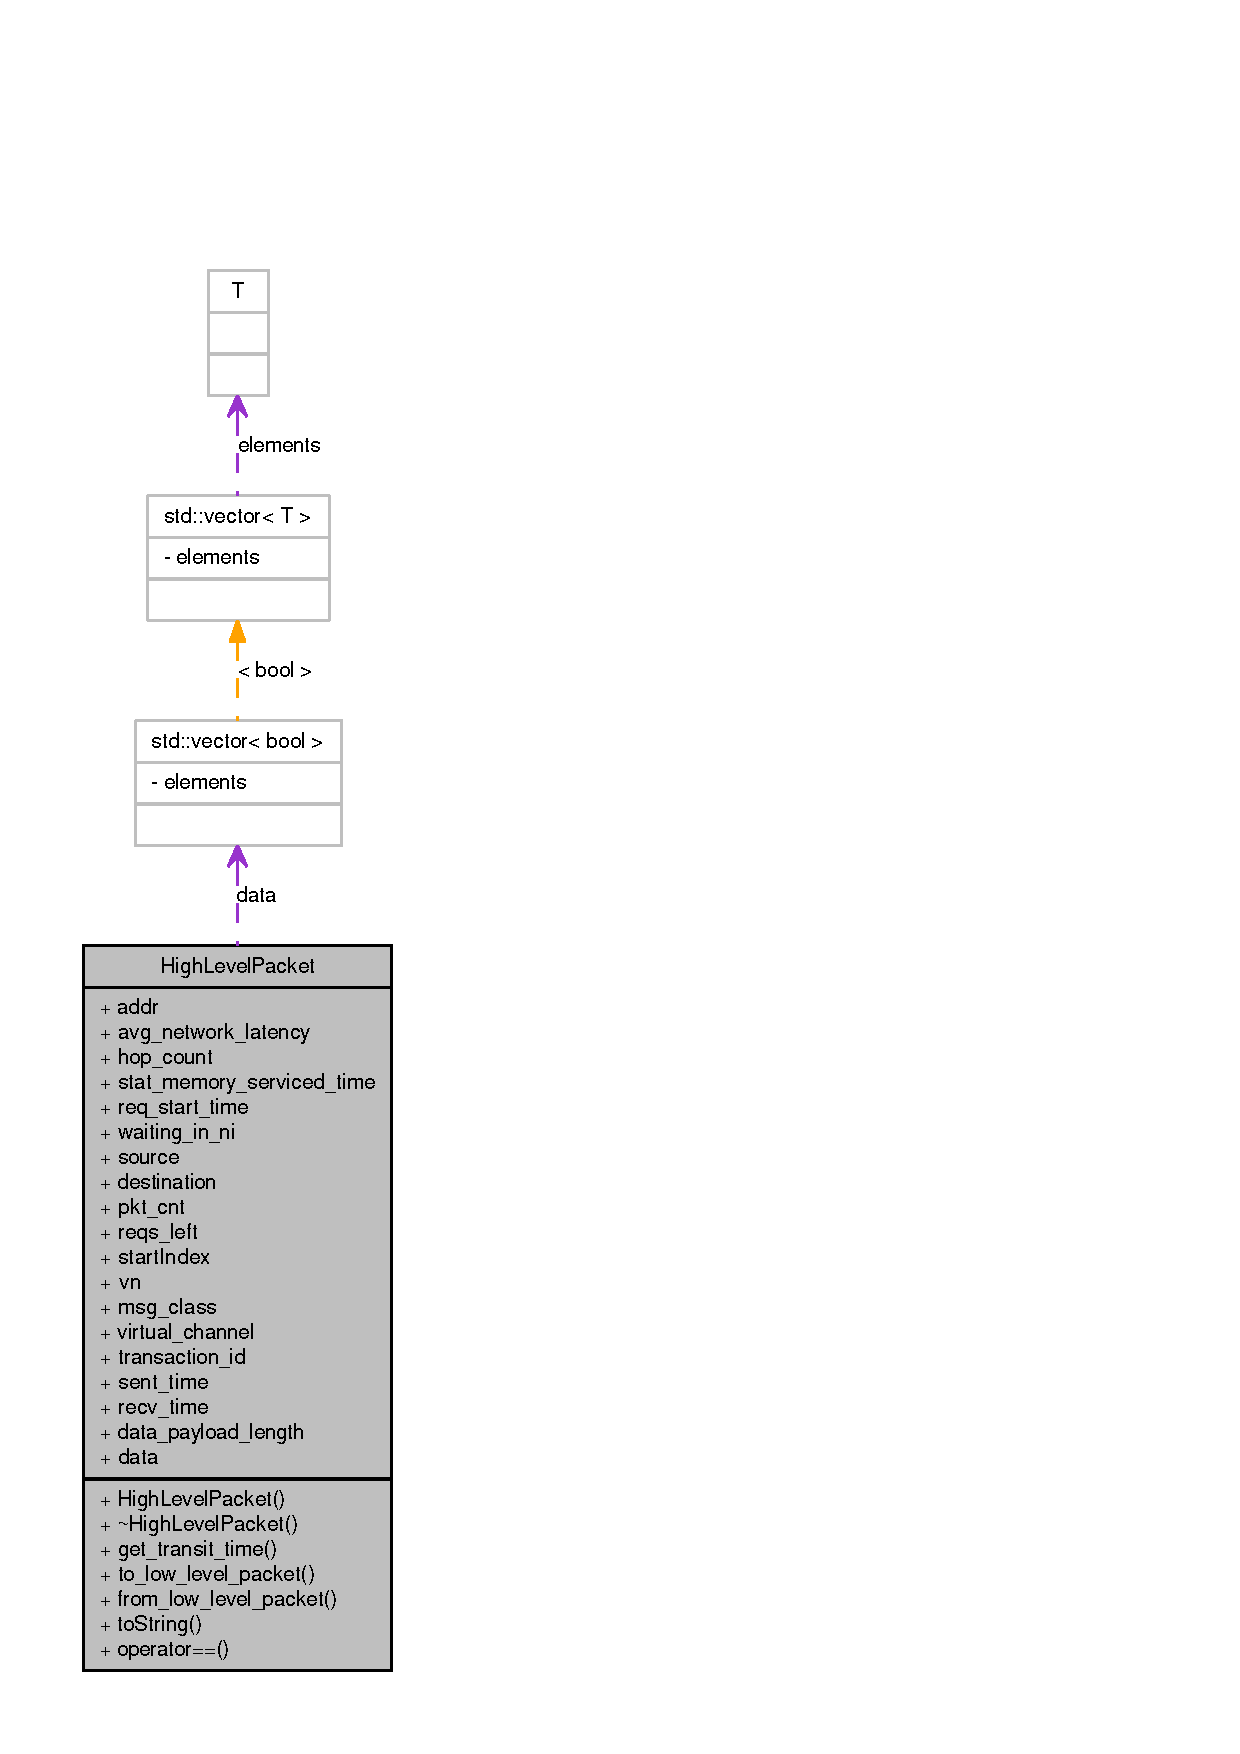
\includegraphics[height=400pt]{classHighLevelPacket__coll__graph}
\end{center}
\end{figure}
\subsection*{Public Member Functions}
\begin{CompactItemize}
\item 
{\bf HighLevelPacket} ()
\item 
{\bf $\sim$HighLevelPacket} ()
\item 
{\bf simTime} {\bf get\_\-transit\_\-time} ()
\item 
void {\bf to\_\-low\_\-level\_\-packet} ({\bf LowLevelPacket} $\ast$llp)
\item 
void {\bf from\_\-low\_\-level\_\-packet} ({\bf LowLevelPacket} $\ast$llp)
\item 
string {\bf toString} () const 
\item 
bool {\bf operator==} (const {\bf HighLevelPacket} $\ast$p)
\end{CompactItemize}
\subsection*{Public Attributes}
\begin{CompactItemize}
\item 
{\bf ullint} {\bf addr}
\item 
double {\bf avg\_\-network\_\-latency}
\item 
unsigned int {\bf hop\_\-count}
\item 
unsigned int {\bf stat\_\-memory\_\-serviced\_\-time}
\item 
{\bf ullint} {\bf req\_\-start\_\-time}
\item 
{\bf ullint} {\bf waiting\_\-in\_\-ni}
\item 
{\bf uint} {\bf source}
\item 
{\bf uint} {\bf destination}
\item 
{\bf uint} {\bf pkt\_\-cnt}
\item 
int {\bf reqs\_\-left}
\item 
{\bf uint} {\bf startIndex}
\item 
{\bf virtual\_\-network} {\bf vn}
\item 
{\bf message\_\-class} {\bf msg\_\-class}
\item 
{\bf uint} {\bf virtual\_\-channel}
\item 
{\bf uint} {\bf transaction\_\-id}
\item 
{\bf simTime} {\bf sent\_\-time}
\item 
{\bf simTime} {\bf recv\_\-time}
\item 
unsigned int {\bf data\_\-payload\_\-length}
\item 
vector$<$ bool $>$ {\bf data}
\end{CompactItemize}


\subsection{Detailed Description}


Definition at line 40 of file highLevelPacket.h.

\subsection{Constructor \& Destructor Documentation}
\index{HighLevelPacket@{HighLevelPacket}!HighLevelPacket@{HighLevelPacket}}
\index{HighLevelPacket@{HighLevelPacket}!HighLevelPacket@{HighLevelPacket}}
\subsubsection[{HighLevelPacket}]{\setlength{\rightskip}{0pt plus 5cm}HighLevelPacket::HighLevelPacket ()}\label{classHighLevelPacket_e6f7a4ec429537928d24f6a2199a3f8d}




Definition at line 31 of file highLevelPacket.cc.

References avg\_\-network\_\-latency, data\_\-payload\_\-length, destination, hop\_\-count, INVALID\_\-PKT, msg\_\-class, Simulator::Now(), pkt\_\-cnt, recv\_\-time, req\_\-start\_\-time, reqs\_\-left, sent\_\-time, source, startIndex, stat\_\-memory\_\-serviced\_\-time, transaction\_\-id, virtual\_\-channel, vn, VN0, and waiting\_\-in\_\-ni.\index{HighLevelPacket@{HighLevelPacket}!$\sim$HighLevelPacket@{$\sim$HighLevelPacket}}
\index{$\sim$HighLevelPacket@{$\sim$HighLevelPacket}!HighLevelPacket@{HighLevelPacket}}
\subsubsection[{$\sim$HighLevelPacket}]{\setlength{\rightskip}{0pt plus 5cm}HighLevelPacket::$\sim$HighLevelPacket ()}\label{classHighLevelPacket_dc29e5ebbbb6e7c3b1d1a53b0ea14142}




Definition at line 52 of file highLevelPacket.cc.

References data.

\subsection{Member Function Documentation}
\index{HighLevelPacket@{HighLevelPacket}!from\_\-low\_\-level\_\-packet@{from\_\-low\_\-level\_\-packet}}
\index{from\_\-low\_\-level\_\-packet@{from\_\-low\_\-level\_\-packet}!HighLevelPacket@{HighLevelPacket}}
\subsubsection[{from\_\-low\_\-level\_\-packet}]{\setlength{\rightskip}{0pt plus 5cm}void HighLevelPacket::from\_\-low\_\-level\_\-packet ({\bf LowLevelPacket} $\ast$ {\em llp})}\label{classHighLevelPacket_6a4e25020ea0c66aab015e9c2a2c8c85}




Definition at line 190 of file highLevelPacket.cc.

References LowLevelPacket::addr, addr, LowLevelPacket::avg\_\-network\_\-latency, avg\_\-network\_\-latency, LowLevelPacket::control\_\-bits, data, data\_\-payload\_\-length, LowLevelPacket::destination, destination, LowLevelPacket::flits, LowLevelPacket::hop\_\-count, hop\_\-count, LowLevelPacket::length, LowLevelPacket::msg\_\-class, msg\_\-class, LowLevelPacket::payload, LowLevelPacket::pkt\_\-cnt, pkt\_\-cnt, LowLevelPacket::req\_\-start\_\-time, req\_\-start\_\-time, LowLevelPacket::sent\_\-time, sent\_\-time, LowLevelPacket::source, source, LowLevelPacket::stat\_\-memory\_\-serviced\_\-time, stat\_\-memory\_\-serviced\_\-time, LowLevelPacket::transaction\_\-id, transaction\_\-id, LowLevelPacket::virtual\_\-channel, virtual\_\-channel, vn, VN0, VN1, VN2, LowLevelPacket::waiting\_\-in\_\-ni, and waiting\_\-in\_\-ni.

Referenced by GenericInterfaceVcs::handle\_\-tick\_\-event(), and GenericInterface::handle\_\-tick\_\-event().

Here is the caller graph for this function:\nopagebreak
\begin{figure}[H]
\begin{center}
\leavevmode
\includegraphics[width=420pt]{classHighLevelPacket_6a4e25020ea0c66aab015e9c2a2c8c85_icgraph}
\end{center}
\end{figure}
\index{HighLevelPacket@{HighLevelPacket}!get\_\-transit\_\-time@{get\_\-transit\_\-time}}
\index{get\_\-transit\_\-time@{get\_\-transit\_\-time}!HighLevelPacket@{HighLevelPacket}}
\subsubsection[{get\_\-transit\_\-time}]{\setlength{\rightskip}{0pt plus 5cm}{\bf simTime} HighLevelPacket::get\_\-transit\_\-time ()}\label{classHighLevelPacket_0ddd2a5fd2195c2ce43198c82163522c}




Definition at line 75 of file highLevelPacket.cc.

References recv\_\-time, and sent\_\-time.\index{HighLevelPacket@{HighLevelPacket}!operator==@{operator==}}
\index{operator==@{operator==}!HighLevelPacket@{HighLevelPacket}}
\subsubsection[{operator==}]{\setlength{\rightskip}{0pt plus 5cm}bool HighLevelPacket::operator== (const {\bf HighLevelPacket} $\ast$ {\em p})}\label{classHighLevelPacket_08e3560b71bab8b1ff31844d8ddff819}




Definition at line 80 of file highLevelPacket.cc.

References source, and transaction\_\-id.\index{HighLevelPacket@{HighLevelPacket}!to\_\-low\_\-level\_\-packet@{to\_\-low\_\-level\_\-packet}}
\index{to\_\-low\_\-level\_\-packet@{to\_\-low\_\-level\_\-packet}!HighLevelPacket@{HighLevelPacket}}
\subsubsection[{to\_\-low\_\-level\_\-packet}]{\setlength{\rightskip}{0pt plus 5cm}void HighLevelPacket::to\_\-low\_\-level\_\-packet ({\bf LowLevelPacket} $\ast$ {\em llp})}\label{classHighLevelPacket_03017f87443d346d08e8ebb4281073c1}




Definition at line 92 of file highLevelPacket.cc.

References HeadFlit::addr, addr, LowLevelPacket::addr, HeadFlit::avg\_\-network\_\-latency, avg\_\-network\_\-latency, LowLevelPacket::avg\_\-network\_\-latency, BodyFlit::bf\_\-data, LowLevelPacket::control\_\-bits, HeadFlit::control\_\-bits, CONTROL\_\-VECTOR\_\-SIZE, data, data\_\-payload\_\-length, destination, LowLevelPacket::destination, HeadFlit::dst\_\-address, LowLevelPacket::flits, HeadFlit::hop\_\-count, hop\_\-count, LowLevelPacket::hop\_\-count, Flit::is\_\-single\_\-flit\_\-pkt, HeadFlit::length, LowLevelPacket::length, max\_\-phy\_\-link\_\-bits, HeadFlit::msg\_\-class, msg\_\-class, LowLevelPacket::msg\_\-class, ONE\_\-FLIT\_\-REQ, TailFlit::packet\_\-originated\_\-time, HeadFlit::packet\_\-originated\_\-time, HeadFlit::payload, HeadFlit::pkt\_\-cnt, pkt\_\-cnt, LowLevelPacket::pkt\_\-cnt, BodyFlit::populate\_\-body\_\-flit(), HeadFlit::populate\_\-head\_\-flit(), TailFlit::populate\_\-tail\_\-flit(), PRIORITY\_\-REQ, HeadFlit::req\_\-start\_\-time, req\_\-start\_\-time, LowLevelPacket::req\_\-start\_\-time, REQUEST\_\-PKT, RESPONSE\_\-PKT, sent\_\-time, LowLevelPacket::sent\_\-time, source, LowLevelPacket::source, HeadFlit::src\_\-address, HeadFlit::stat\_\-memory\_\-serviced\_\-time, stat\_\-memory\_\-serviced\_\-time, LowLevelPacket::stat\_\-memory\_\-serviced\_\-time, HeadFlit::transaction\_\-id, transaction\_\-id, LowLevelPacket::transaction\_\-id, Flit::vc, virtual\_\-channel, LowLevelPacket::virtual\_\-channel, vn, waiting\_\-in\_\-ni, HeadFlit::waiting\_\-in\_\-ni, and WRITE\_\-REQ.

Referenced by GenericInterfaceVcs::handle\_\-new\_\-packet\_\-event(), and GenericInterface::handle\_\-new\_\-packet\_\-event().

Here is the caller graph for this function:\nopagebreak
\begin{figure}[H]
\begin{center}
\leavevmode
\includegraphics[width=420pt]{classHighLevelPacket_03017f87443d346d08e8ebb4281073c1_icgraph}
\end{center}
\end{figure}
\index{HighLevelPacket@{HighLevelPacket}!toString@{toString}}
\index{toString@{toString}!HighLevelPacket@{HighLevelPacket}}
\subsubsection[{toString}]{\setlength{\rightskip}{0pt plus 5cm}string HighLevelPacket::toString () const}\label{classHighLevelPacket_a2292ef0554d515cf08aeed8ca46d419}




Definition at line 57 of file highLevelPacket.cc.

References addr, avg\_\-network\_\-latency, data, data\_\-payload\_\-length, destination, hop\_\-count, msg\_\-class, sent\_\-time, source, transaction\_\-id, and virtual\_\-channel.

Referenced by GenericTPGVcs::handle\_\-new\_\-packet\_\-event(), GenericTPG::handle\_\-new\_\-packet\_\-event(), GenericSink::handle\_\-new\_\-packet\_\-event(), GenericFlatMc::handle\_\-new\_\-packet\_\-event(), GenericTPGVcs::handle\_\-out\_\-pull\_\-event(), GenericRPG::handle\_\-out\_\-pull\_\-event(), GenericSink::handle\_\-outpull\_\-event(), and GenericInterface::handle\_\-tick\_\-event().

Here is the caller graph for this function:\nopagebreak
\begin{figure}[H]
\begin{center}
\leavevmode
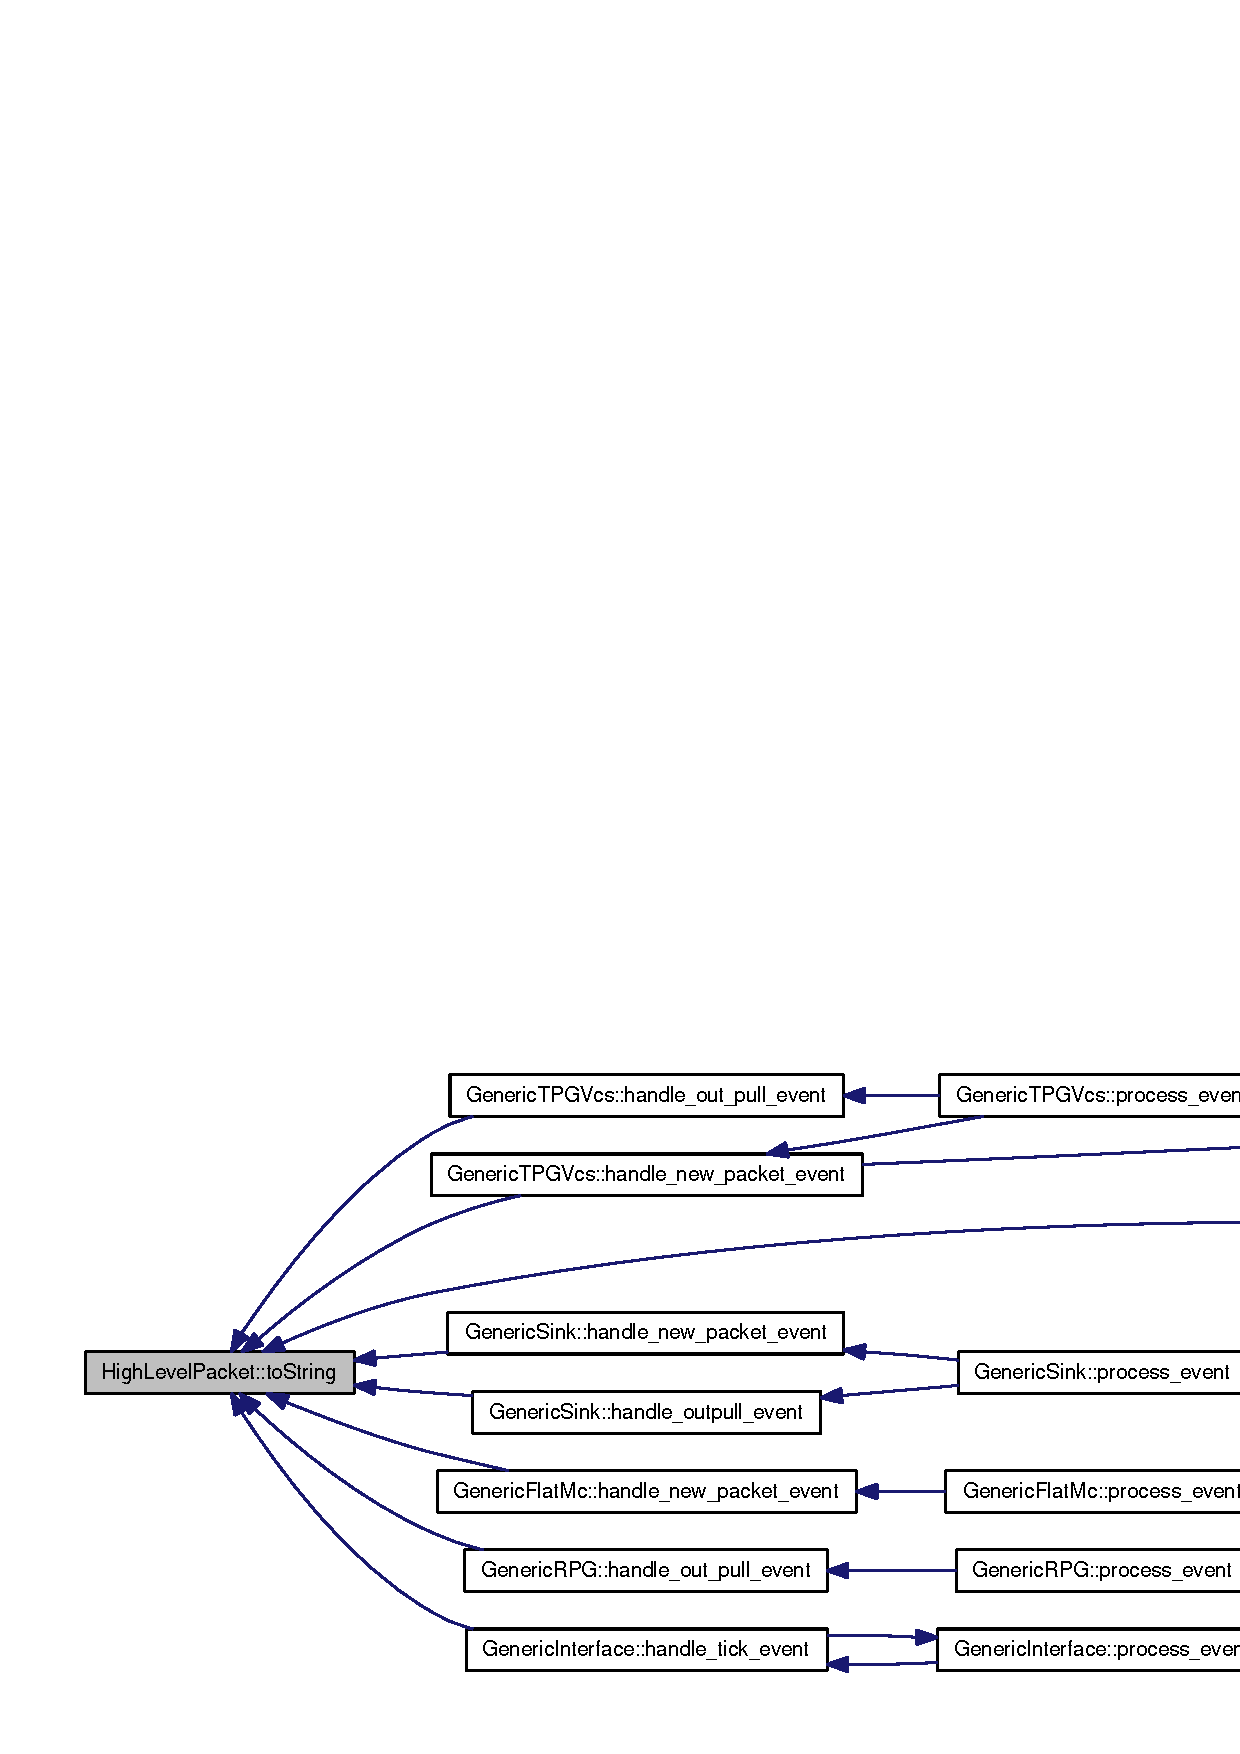
\includegraphics[width=420pt]{classHighLevelPacket_a2292ef0554d515cf08aeed8ca46d419_icgraph}
\end{center}
\end{figure}


\subsection{Member Data Documentation}
\index{HighLevelPacket@{HighLevelPacket}!addr@{addr}}
\index{addr@{addr}!HighLevelPacket@{HighLevelPacket}}
\subsubsection[{addr}]{\setlength{\rightskip}{0pt plus 5cm}{\bf ullint} {\bf HighLevelPacket::addr}}\label{classHighLevelPacket_64f74b9238b8a606a82e41da4d93de93}




Definition at line 61 of file highLevelPacket.h.

Referenced by uncore\_\-t::enqueue(), from\_\-low\_\-level\_\-packet(), GenericInterfaceVcs::handle\_\-new\_\-packet\_\-event(), NI::handle\_\-out\_\-pull\_\-event(), GenericTPGVcs::handle\_\-out\_\-pull\_\-event(), GenericTPG::handle\_\-out\_\-pull\_\-event(), GenericInterfaceVcs::handle\_\-tick\_\-event(), to\_\-low\_\-level\_\-packet(), and toString().\index{HighLevelPacket@{HighLevelPacket}!avg\_\-network\_\-latency@{avg\_\-network\_\-latency}}
\index{avg\_\-network\_\-latency@{avg\_\-network\_\-latency}!HighLevelPacket@{HighLevelPacket}}
\subsubsection[{avg\_\-network\_\-latency}]{\setlength{\rightskip}{0pt plus 5cm}double {\bf HighLevelPacket::avg\_\-network\_\-latency}}\label{classHighLevelPacket_6586c04ecd2c2c5ad01f0f4433f2b77a}




Definition at line 64 of file highLevelPacket.h.

Referenced by from\_\-low\_\-level\_\-packet(), uncore\_\-t::handle\_\-new\_\-packet\_\-event(), NI::handle\_\-new\_\-packet\_\-event(), GenericTPGVcs::handle\_\-new\_\-packet\_\-event(), GenericTPG::handle\_\-new\_\-packet\_\-event(), NI::handle\_\-out\_\-pull\_\-event(), GenericInterfaceVcs::handle\_\-tick\_\-event(), GenericInterface::handle\_\-tick\_\-event(), HighLevelPacket(), to\_\-low\_\-level\_\-packet(), and toString().\index{HighLevelPacket@{HighLevelPacket}!data@{data}}
\index{data@{data}!HighLevelPacket@{HighLevelPacket}}
\subsubsection[{data}]{\setlength{\rightskip}{0pt plus 5cm}vector$<$bool$>$ {\bf HighLevelPacket::data}}\label{classHighLevelPacket_340b7688df206e49a62301e2dae093de}




Definition at line 82 of file highLevelPacket.h.

Referenced by uncore\_\-t::convertFromBitStream(), NI::convertFromBitStream(), GenericTPGVcs::convertFromBitStream(), GenericTPG::convertFromBitStream(), GenericFlatMc::convertFromBitStream(), uncore\_\-t::convertToBitStream(), NI::convertToBitStream(), GenericTPGVcs::convertToBitStream(), GenericTPG::convertToBitStream(), from\_\-low\_\-level\_\-packet(), GenericRPG::handle\_\-out\_\-pull\_\-event(), GenericFlatMc::handle\_\-out\_\-pull\_\-event(), to\_\-low\_\-level\_\-packet(), toString(), and $\sim$HighLevelPacket().\index{HighLevelPacket@{HighLevelPacket}!data\_\-payload\_\-length@{data\_\-payload\_\-length}}
\index{data\_\-payload\_\-length@{data\_\-payload\_\-length}!HighLevelPacket@{HighLevelPacket}}
\subsubsection[{data\_\-payload\_\-length}]{\setlength{\rightskip}{0pt plus 5cm}unsigned int {\bf HighLevelPacket::data\_\-payload\_\-length}}\label{classHighLevelPacket_c7bf05e9b1560991d60ca12fd0d309a3}




Definition at line 81 of file highLevelPacket.h.

Referenced by uncore\_\-t::convertToBitStream(), NI::convertToBitStream(), GenericTPGVcs::convertToBitStream(), GenericTPG::convertToBitStream(), from\_\-low\_\-level\_\-packet(), GenericRPG::handle\_\-out\_\-pull\_\-event(), GenericFlatMc::handle\_\-out\_\-pull\_\-event(), HighLevelPacket(), to\_\-low\_\-level\_\-packet(), and toString().\index{HighLevelPacket@{HighLevelPacket}!destination@{destination}}
\index{destination@{destination}!HighLevelPacket@{HighLevelPacket}}
\subsubsection[{destination}]{\setlength{\rightskip}{0pt plus 5cm}{\bf uint} {\bf HighLevelPacket::destination}}\label{classHighLevelPacket_abe7a75c784f1824211ba194819e0d4e}




Definition at line 71 of file highLevelPacket.h.

Referenced by uncore\_\-t::enqueue(), from\_\-low\_\-level\_\-packet(), NI::handle\_\-out\_\-pull\_\-event(), GenericTPGVcs::handle\_\-out\_\-pull\_\-event(), GenericTPG::handle\_\-out\_\-pull\_\-event(), GenericRPG::handle\_\-out\_\-pull\_\-event(), GenericFlatMc::handle\_\-out\_\-pull\_\-event(), GenericSink::handle\_\-outpull\_\-event(), HighLevelPacket(), to\_\-low\_\-level\_\-packet(), and toString().\index{HighLevelPacket@{HighLevelPacket}!hop\_\-count@{hop\_\-count}}
\index{hop\_\-count@{hop\_\-count}!HighLevelPacket@{HighLevelPacket}}
\subsubsection[{hop\_\-count}]{\setlength{\rightskip}{0pt plus 5cm}unsigned int {\bf HighLevelPacket::hop\_\-count}}\label{classHighLevelPacket_ffa29cc3a49b36a798ae083a6f80f8e5}




Definition at line 65 of file highLevelPacket.h.

Referenced by from\_\-low\_\-level\_\-packet(), uncore\_\-t::handle\_\-new\_\-packet\_\-event(), NI::handle\_\-new\_\-packet\_\-event(), GenericTPGVcs::handle\_\-new\_\-packet\_\-event(), GenericTPG::handle\_\-new\_\-packet\_\-event(), NI::handle\_\-out\_\-pull\_\-event(), GenericInterfaceVcs::handle\_\-tick\_\-event(), GenericInterface::handle\_\-tick\_\-event(), HighLevelPacket(), to\_\-low\_\-level\_\-packet(), and toString().\index{HighLevelPacket@{HighLevelPacket}!msg\_\-class@{msg\_\-class}}
\index{msg\_\-class@{msg\_\-class}!HighLevelPacket@{HighLevelPacket}}
\subsubsection[{msg\_\-class}]{\setlength{\rightskip}{0pt plus 5cm}{\bf message\_\-class} {\bf HighLevelPacket::msg\_\-class}}\label{classHighLevelPacket_e46f274428c73774b8ab21ca885b84ec}




Definition at line 76 of file highLevelPacket.h.

Referenced by uncore\_\-t::convertToBitStream(), GenericTPGVcs::convertToBitStream(), GenericTPG::convertToBitStream(), from\_\-low\_\-level\_\-packet(), NI::handle\_\-out\_\-pull\_\-event(), GenericFlatMc::handle\_\-out\_\-pull\_\-event(), HighLevelPacket(), to\_\-low\_\-level\_\-packet(), and toString().\index{HighLevelPacket@{HighLevelPacket}!pkt\_\-cnt@{pkt\_\-cnt}}
\index{pkt\_\-cnt@{pkt\_\-cnt}!HighLevelPacket@{HighLevelPacket}}
\subsubsection[{pkt\_\-cnt}]{\setlength{\rightskip}{0pt plus 5cm}{\bf uint} {\bf HighLevelPacket::pkt\_\-cnt}}\label{classHighLevelPacket_9e92e51a445389b6c84874638582c156}




Definition at line 72 of file highLevelPacket.h.

Referenced by from\_\-low\_\-level\_\-packet(), HighLevelPacket(), and to\_\-low\_\-level\_\-packet().\index{HighLevelPacket@{HighLevelPacket}!recv\_\-time@{recv\_\-time}}
\index{recv\_\-time@{recv\_\-time}!HighLevelPacket@{HighLevelPacket}}
\subsubsection[{recv\_\-time}]{\setlength{\rightskip}{0pt plus 5cm}{\bf simTime} {\bf HighLevelPacket::recv\_\-time}}\label{classHighLevelPacket_5de1d4d144aa5e9fdac1a3988384d92f}




Definition at line 80 of file highLevelPacket.h.

Referenced by get\_\-transit\_\-time(), NI::handle\_\-new\_\-packet\_\-event(), NI::handle\_\-out\_\-pull\_\-event(), GenericInterfaceVcs::handle\_\-tick\_\-event(), GenericInterface::handle\_\-tick\_\-event(), and HighLevelPacket().\index{HighLevelPacket@{HighLevelPacket}!req\_\-start\_\-time@{req\_\-start\_\-time}}
\index{req\_\-start\_\-time@{req\_\-start\_\-time}!HighLevelPacket@{HighLevelPacket}}
\subsubsection[{req\_\-start\_\-time}]{\setlength{\rightskip}{0pt plus 5cm}{\bf ullint} {\bf HighLevelPacket::req\_\-start\_\-time}}\label{classHighLevelPacket_9976d52a0c6566b9227154d4badcfb57}




Definition at line 67 of file highLevelPacket.h.

Referenced by uncore\_\-t::enqueue(), from\_\-low\_\-level\_\-packet(), uncore\_\-t::handle\_\-new\_\-packet\_\-event(), NI::handle\_\-new\_\-packet\_\-event(), GenericTPGVcs::handle\_\-new\_\-packet\_\-event(), GenericTPG::handle\_\-new\_\-packet\_\-event(), NI::handle\_\-out\_\-pull\_\-event(), GenericTPGVcs::handle\_\-out\_\-pull\_\-event(), GenericTPG::handle\_\-out\_\-pull\_\-event(), GenericInterfaceVcs::handle\_\-tick\_\-event(), GenericInterface::handle\_\-tick\_\-event(), HighLevelPacket(), and to\_\-low\_\-level\_\-packet().\index{HighLevelPacket@{HighLevelPacket}!reqs\_\-left@{reqs\_\-left}}
\index{reqs\_\-left@{reqs\_\-left}!HighLevelPacket@{HighLevelPacket}}
\subsubsection[{reqs\_\-left}]{\setlength{\rightskip}{0pt plus 5cm}int {\bf HighLevelPacket::reqs\_\-left}}\label{classHighLevelPacket_304a1a4171dd986e5081ba7f64cf1257}




Definition at line 73 of file highLevelPacket.h.

Referenced by HighLevelPacket().\index{HighLevelPacket@{HighLevelPacket}!sent\_\-time@{sent\_\-time}}
\index{sent\_\-time@{sent\_\-time}!HighLevelPacket@{HighLevelPacket}}
\subsubsection[{sent\_\-time}]{\setlength{\rightskip}{0pt plus 5cm}{\bf simTime} {\bf HighLevelPacket::sent\_\-time}}\label{classHighLevelPacket_eed2f14fb0b689f35a92c054a831867c}




Definition at line 79 of file highLevelPacket.h.

Referenced by uncore\_\-t::convertToBitStream(), GenericTPGVcs::convertToBitStream(), GenericTPG::convertToBitStream(), uncore\_\-t::enqueue(), from\_\-low\_\-level\_\-packet(), get\_\-transit\_\-time(), uncore\_\-t::handle\_\-new\_\-packet\_\-event(), GenericTPGVcs::handle\_\-new\_\-packet\_\-event(), GenericTPG::handle\_\-new\_\-packet\_\-event(), GenericSink::handle\_\-new\_\-packet\_\-event(), GenericRPG::handle\_\-new\_\-packet\_\-event(), GenericFlatMc::handle\_\-new\_\-packet\_\-event(), NI::handle\_\-out\_\-pull\_\-event(), GenericTPGVcs::handle\_\-out\_\-pull\_\-event(), GenericTPG::handle\_\-out\_\-pull\_\-event(), GenericRPG::handle\_\-out\_\-pull\_\-event(), GenericFlatMc::handle\_\-out\_\-pull\_\-event(), GenericSink::handle\_\-outpull\_\-event(), HighLevelPacket(), to\_\-low\_\-level\_\-packet(), and toString().\index{HighLevelPacket@{HighLevelPacket}!source@{source}}
\index{source@{source}!HighLevelPacket@{HighLevelPacket}}
\subsubsection[{source}]{\setlength{\rightskip}{0pt plus 5cm}{\bf uint} {\bf HighLevelPacket::source}}\label{classHighLevelPacket_d09485039d19ea9f0f58697e9fdf6450}




Definition at line 70 of file highLevelPacket.h.

Referenced by uncore\_\-t::convertFromBitStream(), GenericTPGVcs::convertFromBitStream(), GenericTPG::convertFromBitStream(), uncore\_\-t::enqueue(), from\_\-low\_\-level\_\-packet(), NI::handle\_\-out\_\-pull\_\-event(), GenericTPGVcs::handle\_\-out\_\-pull\_\-event(), GenericTPG::handle\_\-out\_\-pull\_\-event(), GenericRPG::handle\_\-out\_\-pull\_\-event(), GenericFlatMc::handle\_\-out\_\-pull\_\-event(), GenericSink::handle\_\-outpull\_\-event(), HighLevelPacket(), operator==(), to\_\-low\_\-level\_\-packet(), and toString().\index{HighLevelPacket@{HighLevelPacket}!startIndex@{startIndex}}
\index{startIndex@{startIndex}!HighLevelPacket@{HighLevelPacket}}
\subsubsection[{startIndex}]{\setlength{\rightskip}{0pt plus 5cm}{\bf uint} {\bf HighLevelPacket::startIndex}}\label{classHighLevelPacket_ec807a7bab73b8adc80d3a3df586a47d}




Definition at line 74 of file highLevelPacket.h.

Referenced by HighLevelPacket().\index{HighLevelPacket@{HighLevelPacket}!stat\_\-memory\_\-serviced\_\-time@{stat\_\-memory\_\-serviced\_\-time}}
\index{stat\_\-memory\_\-serviced\_\-time@{stat\_\-memory\_\-serviced\_\-time}!HighLevelPacket@{HighLevelPacket}}
\subsubsection[{stat\_\-memory\_\-serviced\_\-time}]{\setlength{\rightskip}{0pt plus 5cm}unsigned int {\bf HighLevelPacket::stat\_\-memory\_\-serviced\_\-time}}\label{classHighLevelPacket_9b5cf0352fb4890ab094d21de459474a}




Definition at line 66 of file highLevelPacket.h.

Referenced by from\_\-low\_\-level\_\-packet(), uncore\_\-t::handle\_\-new\_\-packet\_\-event(), GenericTPGVcs::handle\_\-new\_\-packet\_\-event(), GenericTPG::handle\_\-new\_\-packet\_\-event(), NI::handle\_\-out\_\-pull\_\-event(), GenericFlatMc::handle\_\-out\_\-pull\_\-event(), HighLevelPacket(), and to\_\-low\_\-level\_\-packet().\index{HighLevelPacket@{HighLevelPacket}!transaction\_\-id@{transaction\_\-id}}
\index{transaction\_\-id@{transaction\_\-id}!HighLevelPacket@{HighLevelPacket}}
\subsubsection[{transaction\_\-id}]{\setlength{\rightskip}{0pt plus 5cm}{\bf uint} {\bf HighLevelPacket::transaction\_\-id}}\label{classHighLevelPacket_287c21f9e31f882ffe8c8ff353dab087}




Definition at line 78 of file highLevelPacket.h.

Referenced by uncore\_\-t::enqueue(), from\_\-low\_\-level\_\-packet(), NI::handle\_\-out\_\-pull\_\-event(), GenericTPGVcs::handle\_\-out\_\-pull\_\-event(), GenericTPG::handle\_\-out\_\-pull\_\-event(), GenericRPG::handle\_\-out\_\-pull\_\-event(), GenericFlatMc::handle\_\-out\_\-pull\_\-event(), GenericSink::handle\_\-outpull\_\-event(), HighLevelPacket(), operator==(), to\_\-low\_\-level\_\-packet(), and toString().\index{HighLevelPacket@{HighLevelPacket}!virtual\_\-channel@{virtual\_\-channel}}
\index{virtual\_\-channel@{virtual\_\-channel}!HighLevelPacket@{HighLevelPacket}}
\subsubsection[{virtual\_\-channel}]{\setlength{\rightskip}{0pt plus 5cm}{\bf uint} {\bf HighLevelPacket::virtual\_\-channel}}\label{classHighLevelPacket_0e369f54800e9bb403f8277b94cbaa96}




Definition at line 77 of file highLevelPacket.h.

Referenced by uncore\_\-t::enqueue(), from\_\-low\_\-level\_\-packet(), uncore\_\-t::handle\_\-new\_\-packet\_\-event(), NI::handle\_\-new\_\-packet\_\-event(), GenericTPGVcs::handle\_\-new\_\-packet\_\-event(), GenericSink::handle\_\-new\_\-packet\_\-event(), GenericRPG::handle\_\-new\_\-packet\_\-event(), GenericInterfaceVcs::handle\_\-new\_\-packet\_\-event(), GenericInterface::handle\_\-new\_\-packet\_\-event(), NI::handle\_\-out\_\-pull\_\-event(), GenericTPGVcs::handle\_\-out\_\-pull\_\-event(), GenericTPG::handle\_\-out\_\-pull\_\-event(), GenericRPG::handle\_\-out\_\-pull\_\-event(), GenericFlatMc::handle\_\-out\_\-pull\_\-event(), GenericSink::handle\_\-outpull\_\-event(), GenericInterfaceVcs::handle\_\-tick\_\-event(), HighLevelPacket(), to\_\-low\_\-level\_\-packet(), and toString().\index{HighLevelPacket@{HighLevelPacket}!vn@{vn}}
\index{vn@{vn}!HighLevelPacket@{HighLevelPacket}}
\subsubsection[{vn}]{\setlength{\rightskip}{0pt plus 5cm}{\bf virtual\_\-network} {\bf HighLevelPacket::vn}}\label{classHighLevelPacket_0e554b43c609ab77758300f332679a29}




Definition at line 75 of file highLevelPacket.h.

Referenced by from\_\-low\_\-level\_\-packet(), HighLevelPacket(), and to\_\-low\_\-level\_\-packet().\index{HighLevelPacket@{HighLevelPacket}!waiting\_\-in\_\-ni@{waiting\_\-in\_\-ni}}
\index{waiting\_\-in\_\-ni@{waiting\_\-in\_\-ni}!HighLevelPacket@{HighLevelPacket}}
\subsubsection[{waiting\_\-in\_\-ni}]{\setlength{\rightskip}{0pt plus 5cm}{\bf ullint} {\bf HighLevelPacket::waiting\_\-in\_\-ni}}\label{classHighLevelPacket_80531eda576b228669b9ed662e4863fc}




Definition at line 68 of file highLevelPacket.h.

Referenced by from\_\-low\_\-level\_\-packet(), uncore\_\-t::handle\_\-new\_\-packet\_\-event(), GenericTPGVcs::handle\_\-new\_\-packet\_\-event(), GenericTPG::handle\_\-new\_\-packet\_\-event(), NI::handle\_\-out\_\-pull\_\-event(), GenericFlatMc::handle\_\-out\_\-pull\_\-event(), GenericInterfaceVcs::handle\_\-tick\_\-event(), GenericInterface::handle\_\-tick\_\-event(), HighLevelPacket(), and to\_\-low\_\-level\_\-packet().

The documentation for this class was generated from the following files:\begin{CompactItemize}
\item 
{\bf highLevelPacket.h}\item 
{\bf highLevelPacket.cc}\end{CompactItemize}
